\chapter{Contexte}
% parler de la saillance, fixation, saccades, dataset
\par
Le stage a commencé par de la documentation en rapport avec le sujet de stage. N'ayant pas d'accès à un poste la première semaine de stage, Olivier m'a donné quelques documents introduisant des notions importantes sur le regard humain et la saillance. Ce sont des domaines plutôt liés à l'anatomie et la psychologie mais qu'il est important de comprendre si l'on veut pouvoir interpréter les résultats obtenus en sortie des scripts.
\par
Je vais vous expliquer ici les notions fondamentales qui permettent de comprendre le regard humain et comment il est possible de le mesurer pour l'analyser.

\section{Fixation et saccade}
\label{section:fix_sacc}
\par
Le regard est une alternance entre des périodes où l'\oe{}il reste relativement stationnaire, que l'on appelle "\textbf{fixations}", et de courtes périodes de plus grande mobilité, que l'on appelle "\textbf{saccades}"\cite{gaze}. Ce sont des notions qui ont été décrites pour la première fois en 1879 par Javal et Lamare. Il a été possible d'établir des mesures sur le mouvement des yeux deux décades plus tard (Erdmann et Dodge 1898). Ces mesures ont ouvert le champs aux possibilités d'expérimentation sur la psychologie liée au mouvement des yeux. Cela a permis de mieux comprendre le processus d'analyse quand quelqu'un lit, résoud un problème, regarde un film ou quand quelqu'un regarde une peinture.

\par
Chaque fixation est reliée à une autre fixation par une saccade. Ainsi le regard d'une personne dans le temps est donc constitué d'une succession de fixations et de saccades qui forment une chaine. On appelle cela le \textbf{chemin visuel}. C'est en analysant le chemin visuel que l'on est capable de comprendre comment un individu regarde une peinture ou tout autre élément visuel.

\begin{figure}[!ht]
    \centering
    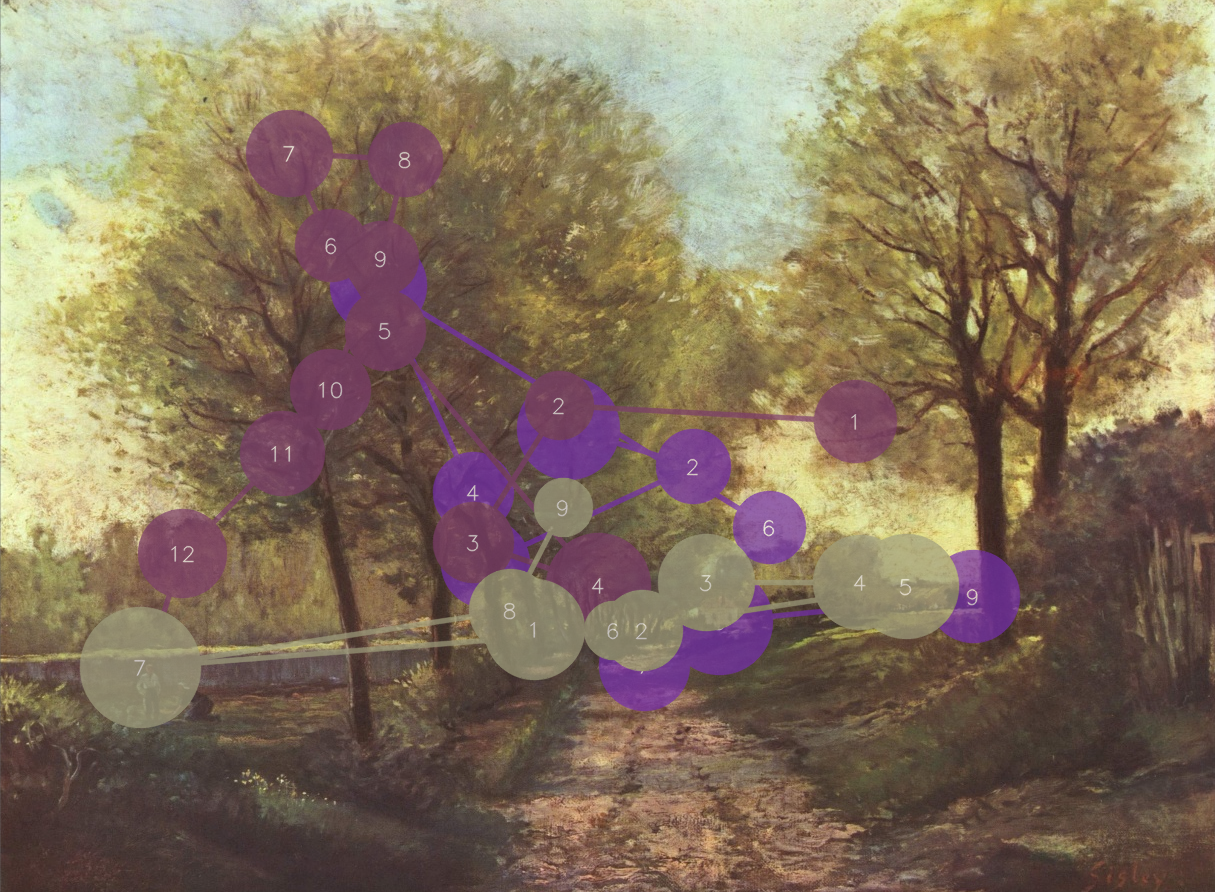
\includegraphics[width=0.7\linewidth]{datas/exemple_scanpaths2.png}
    \caption{Exemple de chemins visuels de 3 observateurs différents.}
    \label{ex_scanpath}
\end{figure}

\par
Sur l'image \ref{ex_scanpath} (\emph{Avenue of trees in a small town}, A. Sisley, 1866) on peut voir l'exemple d'une représentation de chemins visuels de trois observateurs différents distingués chacun par une couleur différente. Sur cette image chaque fixation est représentée par un cercle numéroté qui correspond à son positionnement dans le parcours du regard. La taille des cercles dépend de la durée de la fixation en question. Ici chaque fixation est reliée à une autre fixation par un trait qui représente une saccade.

\section{Saillance et carte de saillance}
\par
Sur l'exemple précédent il est facile de remarquer que chaque individu aborde la peinture avec un regard différent d'un autre. Cependant il est très important de noter qu'il y a des similarités dans les zones regardées. Il y a des endroits de la peintures que les trois observateurs ont regardé, comme le bout du chemin ou l'arbre de gauche au premier plan, tandis que d'autres endroits sont ignorés, les bordures de la peinture entre autre. Ce sont ces zones plus souvent regardées que l'on appellera des zones saillantes.

\par
La \textbf{saillance} est donc la notion qui définie qu'un élément est facilement remarqué. Elle existe aussi dans le domaine sonore ou linguistique. Ici c'est évidemment la saillance visuelle qui nous intéresse. Un élément dit saillant est donc un élément qui dénote du reste de l'\oe{}uvre et qui attirera le regard de l'observateur. Les critères qui définisse la saillance d'un objet sont régies par deux facteurs important. Le facteur "\textbf{Bottom-up}" basé sur les information simple comme les couleurs, le contraste ou la luminosité. Le facteur "\textbf{Top-down}" lui est basé sur des informations propres à l'observateur. Il peut être influencé par une tâche à accomplir, par sa culture, ses connaissances, son âge...\ C'est à partir de tous ces éléments que l'on peut déduire une forte connexion entre le mouvement des yeux, ou le chemin visuel, et la saillance d'une peinture.

\par
De cette relation on va pouvoir, à partir du chemin visuel de plusieurs observateurs, générer une \textbf{carte de saillance} (voir image \ref{ex_saliency_map}). Celle-ci va nous permettre de mettre en évidence les éléments saillants d'une image. Elle est obtenue en moyennant les points de fixations de différents observateurs. 

\begin{figure}[!ht]
    \centering
    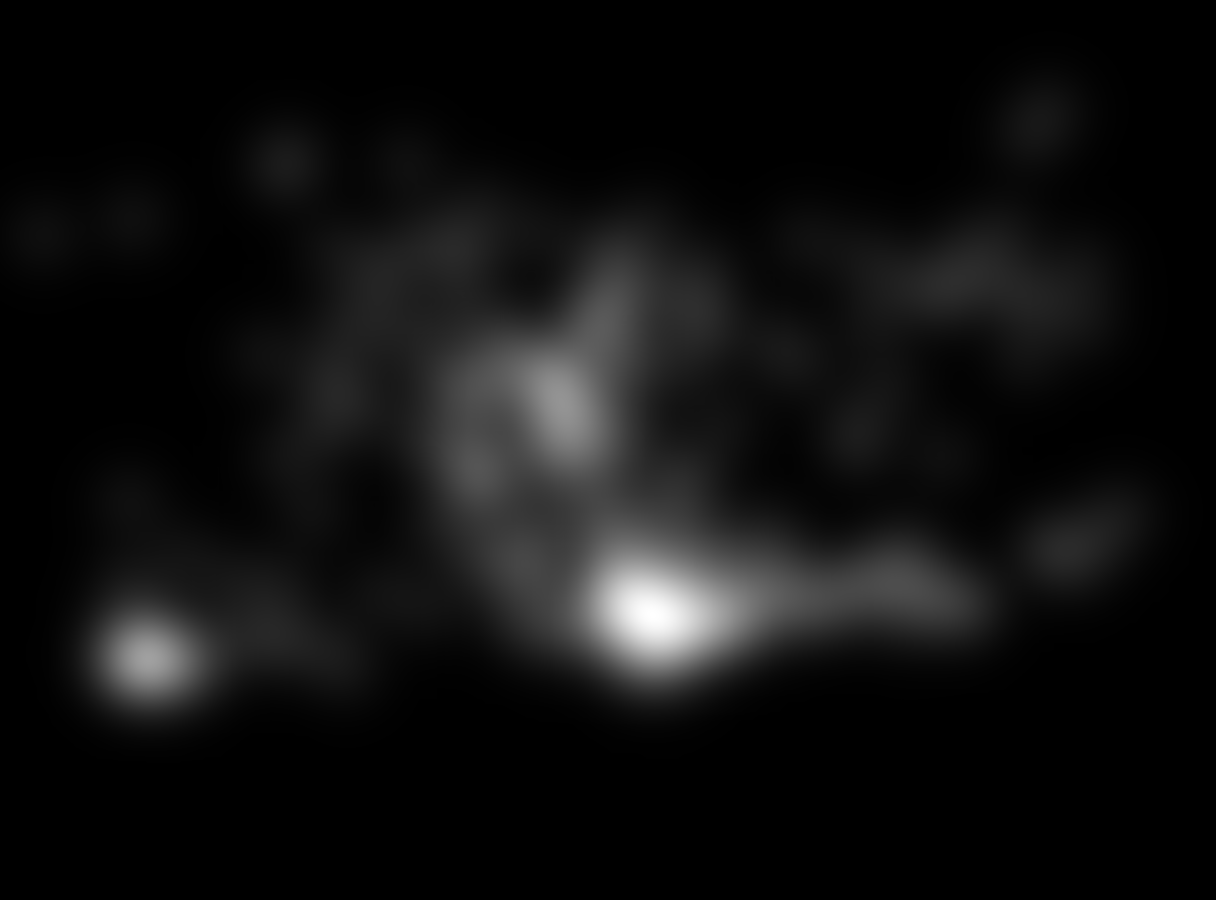
\includegraphics[width=0.7\linewidth]{datas/exemple_saliency_map.png}
    \caption{Exemple de carte de saillance}
    \label{ex_saliency_map}
\end{figure}

\par
Si on superpose la carte de saillance et la peinture associée on peut facilement voir quels sont les éléments saillants de l'\oe{}uvre (voir image \ref{saliency_map_transparency}). Ici la carte de saillance nous révèle que le village au bout du chemin, les deux personnages en bas à gauche et la végétation au premier plan sont les éléments saillants de l'\oe{}uvre.

\begin{figure}[!ht]
    \centering
    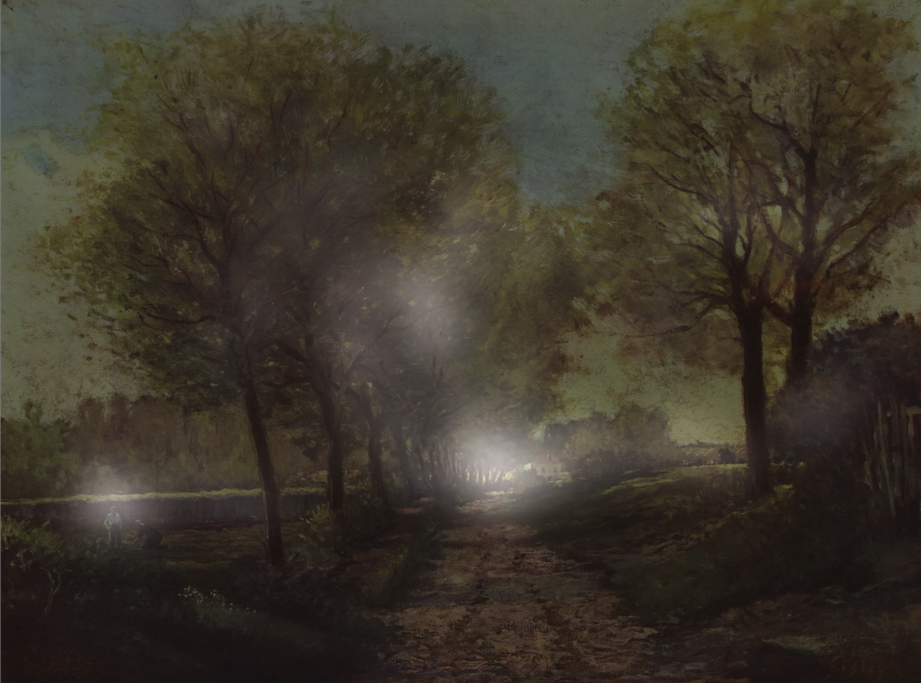
\includegraphics[width=0.7\linewidth]{datas/exemple_saliency_map_transparency.png}
    \caption{Carte de saillance et peinture superposées}
    \label{saliency_map_transparency}
\end{figure}

\par
Mon but lors de ce stage sera d'entrainer un réseau de neurones capable de générer une carte de saillance avec comme seule entrée une peinture. 

\section{Base de données et oculométrie}
\par
Afin de pouvoir entrainer un réseau de neurones il nous faut une base de données avec des données oculométriques sur des peintures. C'est-à-dire une base de données avec l'enregistrement du chemin visuel de différents observateurs qui regardent une peinture.

\par
La mesure du mouvement des yeux d'une personne est possible grâce à un \textbf{oculomètre} (voir image \ref{oculo}). Cet appareil retranscrit le regard d'un observateur avec une grande précision et peut nous donner des informations comme la position et la durée d'une fixation. Inventé vers la fin du 19\up{ème} siècle, il en existe aujourd'hui des versions électroniques très efficace.

\begin{figure}[!ht]
    \centering
    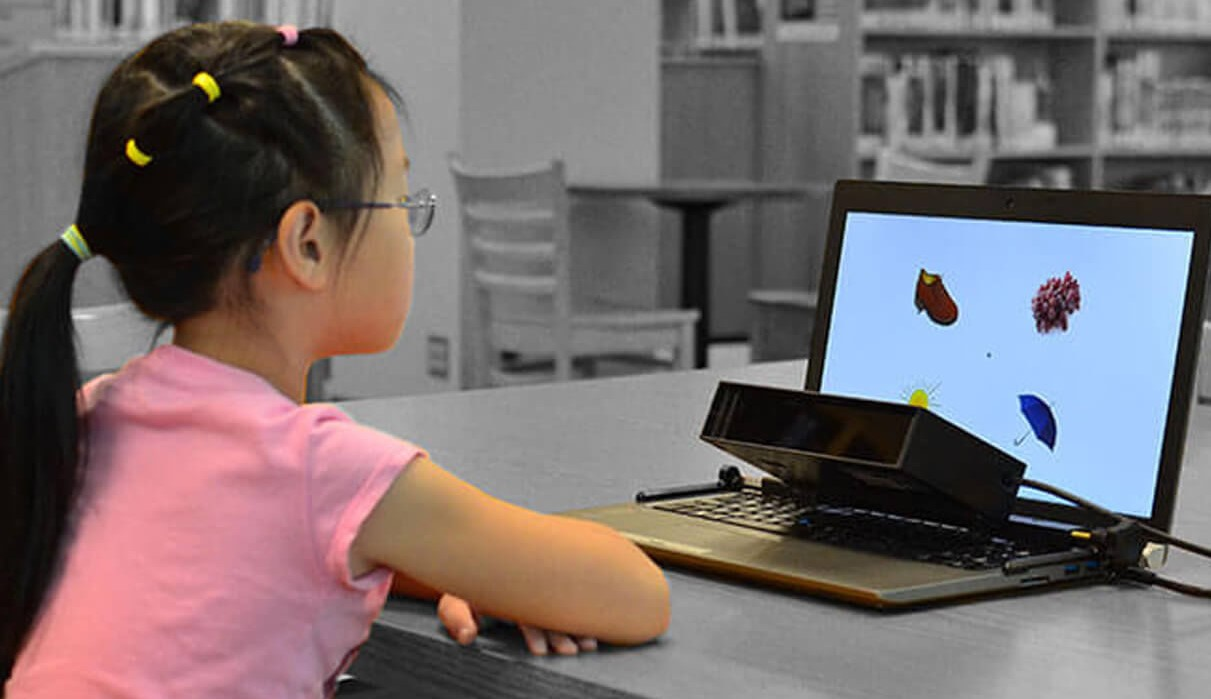
\includegraphics[width=0.7\linewidth]{datas/oculometre.jpg}
    \caption{Exemple d'oculomètre}
    \label{oculo}
\end{figure}

Des étudiants de l'ISTIC ont effectuer un stage sous la direction d'Olivier Le Meur pour constituer une base de données oculométrique de 21 observateurs sur un total de 150 peintures. Ce sont des peintures de 5 grands mouvements artistiques (Fauvisme, Impressionnisme, Réalisme, Romantisme et Pointillisme) avec chacun 3 genres (Nature morte, Nu, Paysage). Chaque participants avait 5 secondes pour regarder une peinture ce qui nous donne des données oculométrique étaler de 5 secondes dans le temps.